Elektronový spin je veličina poněkud záhadná, veličina, která nemá obdoby v~klasickém světe. Do kvantové mechaniky se spin dostal jako experimentální fakt: z~řady experimentů totiž vyplývalo, že kromě orbitálního momentu má elektron ještě nějaký dodatečný moment hybnosti. V~nerelativistické kvantové teorii jeho existenci prostě postulujeme. Elektronový spin ovšem přirozeným způsobem vyplynul ze snahy vytvořit relativistickou kvantovou teorii. Toto téma jde však za rámec našeho stručného textu.

\subsection{Pojem spinu}
\label{kap:PojemSpinu}

Spin je vlastní moment hybnosti částice, kupříkladu elektronu. V~následujících oddílech se stručně seznámíme s~tím, jak se vlastně na existenci spinu přišlo.

V~kapitole~\ref{kap:momenthybnosti} jsme se blíže seznámili s~orbitálním momentem, který je v~klasické fyzice definován vztahem
\begin{equation}
\mathbf{L} \equiv \mathbf{r} \times \mathbf{p} \mbox{,}
\label{rov:Spin1}
\end{equation}
kde $\mathbf{r}$ je kolmá vzdálenost od osy otáčení a $\mathbf{p} = m \mathbf{v}$ je hybnost. Moment hybnosti $\mathbf{L}$ označujeme jako orbitální z~toho důvodu, že objekt, který obíhá okolo daného středu po tzv. orbitu, má nenulový orbitální moment. V~případě atomu si můžeme představit elektron, který obíhá kolem atomového jádra. Protože elektron nese elementární náboj $e$, generuje při svém orbitálním pohybu proudovou smyčku, která vytváří magnetické pole. Sílu takto vzniklého pole měříme pomocí magnetického momentu spojeného s~orbitálním momentem hybnosti
\begin{equation}
\mu_L = -\frac{e}{2m_e}\mathbf{L} \mbox{.}
\label{rov:Spin2}
\end{equation}
Vztah (\ref{rov:Spin2}) je uveden pro případ elektronu -- hmotnost $m_e$ a náboj $e$. Obecně by ve vztahu figurovala hmotnost částice $m$ a náboj částice $q$. 

Uvažujme nyní atom, ve kterém rotuje elektron. Takovýto atom může mít nenulový magnetický moment, který jsme schopni změřit například pomocí vychylování směru atomu v~nehomogenním magnetickém poli. Potenciální energie interakce magnetického momentu s~vnějším magnetickým polem je
\begin{equation}
V_m = - \mu B \cos \theta,
\nonumber
\end{equation}
kde $\mu$ je magnetický moment, $B$ je magnetická indukce vnějšího pole a $\theta$ je úhel, který svírají tyto vektory. Dosazením ze vztahu \eqref{rov:Spin2} dostaneme
\begin{equation}
V_m = \left( \frac{e}{2m_e} \right) LB \cos \theta.
\label{rov:Spin25}
\end{equation}
Význam vnějšího magnetické pole je ten, že určuje experimentálně význačný směr, s~jehož pomocí můžeme určit $L_z$, neboli $z$-ovou složku momentu hybnosti. Z~kapitoly \ref{kap:momenthybnosti} víme, že velikost vektoru momentu hybnosti i jeho $z$-ová složka jsou kvantovány. Pak pro $\cos \theta$ můžeme odvodit (viz obrázek \ref{obr:VektorovyModel})
\begin{equation}
\cos \theta = \frac{m}{\sqrt{l(l+1)}}.
\nonumber
\end{equation}
Výraz \eqref{rov:Spin25} tak můžeme přepsat do tvaru
\begin{equation}
V_m = m \left(\frac{e \hbar}{2 m_e} \right) B,
\label{rov:Spin26}
\end{equation}
kde jsme využili toho, že platí $L = \sqrt{l(l+1)}\hbar$. Výraz v~závorce ve vztahu \eqref{rov:Spin26} se označuje jako Bohrův magneton a má hodnotu $\mu_B = 9,27 \cdot 10^{-24} \joule \tesla^{-1}$. Vidíme, že ve vnějším magnetickém poli závisí energie elektronu na magnetickém kvantovém čísle $m$.

Tak například elektronový stav s~vedlejším kvantovým číslem $l = 1$ (p-orbital) se ve vnějším magnetickém poli rozštěpí do tří různých stavů s~různou energií podle hodnot magnetického kvantového čísla $m = -1, 0, 1$. To vede k~rozštěpení původní jediné spektrální čáry v~atomovém spektru do tripletu, přičemž vzdálenost mezi čárami závisí na velikosti magnetického pole, tj. magnetické indukci $\mathbf{B}$. Štěpení spektrálních čar v~magnetickém poli se nazývá Zeemanův jev po svém objeviteli holandském fyzikovi Zeemanovi, který ho poprvé pozoroval v~roce 1896. Zeemanův jev je tak přímým experimentálním potvrzením prostorového kvantování momentu hybnosti.

Ve skutečnosti se ukázalo, že štěpení atomových hladin v~magnetickém poli může být o~dost složitější, než předpovídala kvantová mechanika. Toto  anomální chování (anomální Zeemanův jev) bylo možno vysvětlit zavedením dodatečného momentu hybnosti elektronu, tedy spinu. Nejjasnější experimentální důkaz existence spinu podal experiment provedený v~roce 1922 Otto Sternem a Walterem Gerlachem. Tento experiment si proto probereme důkladněji.    


\subsection{Sternův - Gerlachův experiment}
\label{kap:SG experiment}

Experimentální aparatura (viz obrázek \ref{obr:SCH-experiment}) Sternova-Gerlachova experimentu sestávala z~pícky, ve které se zahřívaly atomy stříbra. Páry stříbra opouštěly pícku malým otvorem a~vytvářely paprsek atomů. Paprsek procházel nehomogenním magnetickým polem a dopadal na vhodné stínítko, které sloužilo k~vizualizaci výsledků. Předpokladem experimentu je, že atomy stříbra mají nenulový dipólový moment. Atomy s~nenulovým dipólovým momentem interagují s~nehomogenním magnetickým polem a jsou vychýleny z~přímého směru v~závislosti na prostorové orientaci magnetického momentu. Zvolme orientaci nehomogenního magnetického pole ve směru osy $z$. Pak pro sílu, která způsobuje vychýlení atomů z~přímé dráhy platí
\begin{equation}
F_z = - \frac{\partial U}{\partial z } \mbox{,}
\label{rov:Spin5}
\end{equation}
kde $U = - \mu \cdot B = - \mu_z B_z$ je potenciální energie atomů stříbra v~magnetickém poli orientovaném ve směru $z$-ové osy. Proto 
\begin{equation}
F_z = \mu_z \frac{\partial B}{\partial z } \mbox{.}
\label{rov:Spin6}
\end{equation}

\begin{figure} [!ht]
\centering
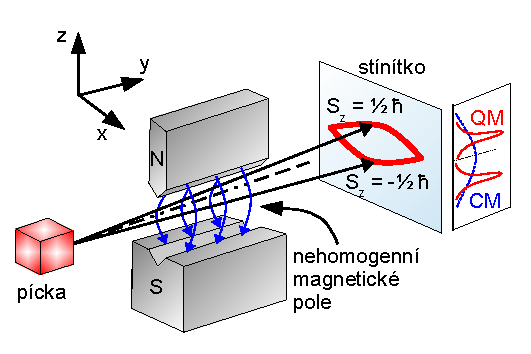
\includegraphics[scale=1]{SGE.pdf}
\caption[Sternův - Gerlachův experiment]{Schématické zobrazení experimentální aparatury, kterou použili Stern s~Gerlachem při experimentu, kterým chtěli prokázat prostorové kvantování orbitálního momentu hybnosti. Ve skutečnosti prokázali existenci spinu, dalšího momentu hybnosti elektronu. Aparatura se skládala z~pícky s~atomy stříbra, které ze zahřály a opouštěly pícku malým otvorem, přičemž tvořily atomový paprsek. Atomy procházely nehomogenním magnetickým polem a~vychylovaly se v~závislosti na prostorové orientaci spinu. Po dopadu na stínítko se vytvořily dvě stopy odpovídající dvěma prostorovým projekcím spinu -- spin nahoru a spin dolů. Dále je zobrazeno porovnání očekávané distribuce dopadů atomů stříbra na stínítko podle klasické (CM) a~kvantové (QM) mechaniky.}
\label{obr:SCH-experiment}
\end{figure}


Podle představ klasické fyziky bude magnetický moment stříbrných atomů orientován v~prostoru zcela náhodně a jeho průmět do osy z~tak bude také nabývat libovolných hodnot od -$|\mu|$ do $|\mu|$. Na stínítku bychom dostali přímou čáru o~velikosti ve směru $z$-ové osy odpovídající dopadům stříbrných atomů. Stříbrné atomy ale dopadaly na stínítko pouze ve dvou bodech, které odpovídaly dipólovému momentu
\begin{equation}
\mu_z = \pm \mu_B, \quad \mu_B = \frac{e\hbar}{2m_e}\mbox{,}
\label{rov:Spin7}
\end{equation}
kde $\mu_B$ je Bohrův magneton. Stern s~Gerlachem byli nadšeni, neboť tento experiment potvrzoval kvantování momentu hybnosti ve směru osy z, jak předpovídala kvantová teorie. Jenže pozornější pohled už ukazuje, že zde něco nesouhlasí.  Atomy stříbra mají 47 elektronů, z~nichž 46 je spárovaných, a tudíž nepřispívají k~orbitálnímu momentu hybnosti. Zbývající 1 nespárovaný elektron má také nulový orbitální mement hybnosti, protože obsazuje $5s$ orbital. Celkový orbitální moment hybnosti atomů stříbra je tedy $\mathbf{L}=0$, a tak neexistuje žádný magnetický moment vyvolaný tímto momentem hybnosti. Můžeme připustit, že onen nespárovaný elektron se z~nějakých důvodu bude nacházet v~p orbitalu. V~této situaci by se ale měl svazek stříbra rozpadat na tři, nikoliv na dva podsvazky. pozorovaný nenulový magnetický moment atomů stříbra musí být vyvolán dalším momentem hybnosti -- spinem. Sternův - Gerlachův experiment tak představuje přímou experimentální metodu umožňující měřit jednu z~komponent spinu, v~našem případě $z$-ovou komponentu. Koncept spinu elektronu byl zaveden až v~roce 1925 holandskými fyziky Georgem Uhlenbeckem a Samuelem Goudsmitem, kteří analyzovali atomová spektra. I~přesto je Sternův - Gerlachův experiment považován za experimentální důkaz existence elektronového spinu.


\subsection{Spin a rotace elektronu kolem své osy}

Samotné slovo "spin" je odvozeno z~anglického slovesa "to spin", tedy točiti se, vířiti, vrtěti se. Odkazuje na představu, že spin je moment hybnosti spojený s~vlastní rotací částice. Takový výklad je ovšem pochybený. Budeme-li si představovat spin jako moment hybnosti spojený s~rotujícím objektem (například pohyb planety Země otáčející se kolem své osy je spojen s~momentem hybnosti, můžeme příslušný moment hybnosti určit pomocí vztahu
\begin{equation}
\mathbf{S} = I \omega \mbox{,}
\label{rov:Spin3}
\end{equation}
kde moment hybnosti  $S$ nazveme spinovým momentem hybnosti či krátce spinem,  $I$ je moment setrvačnosti související s~distribucí hmoty objektu okolo osy rotace a $\omega$ je úhlová rychlost. Spin je vektorová veličina orientovaná v~ose rotace a jeho směr je určen pomocí pravidla pravé ruky. Pakliže je rotující objekt nabitý, jeho rotace opět způsobí vznik magnetického pole. I~zde charakterizujeme magnetické pole magnetickým momentem, tentokráte spojeným se spinovým momentem hybnosti
\begin{equation}
\mu_S = \frac{q}{2m}\mathbf{S} \mbox{,}
\label{rov:Spin4}
\end{equation}
kde $q$ je náboj rotujícího tělesa.

Elementární částice jako je elektron jsou bodové částice a nedá se tak mluvit o~jejich rotaci. To znamená, že moment setrvačnosti jde k~nule, $I \rightarrow 0$, a proto i spin částic se bude blížit nule, $\mathbf{S} \rightarrow 0$. Kdyby tomu tak bylo, elementární částice by neměly žádný dipólový moment související se spinem, což je v~rozporu s~experimentem. Ve snaze zlepšit tuto neshodu můžeme připustit, že elementární částice jsou velmi malé rotující kuličky. Z~experimentů plyne, že poloměry částic jsou $< 10^{-17} \,\mbox{m}$. Aby například elektron s~tímto poloměrem měl příslušnou hodnotu svého spinu, musel by rotovat daleko větší rychlostí, než je rychlost světla. Tento rozpor vede k~tomu, že klasická mechanika při popisu elementárních částic selhává a musíme jí nahradit kvantovou teorií.


\subsection{Spin v~kvantové mechanice}
\label{kap:Spin-QM}

Pojďme nyní zavést spin do formalismu kvantové mechaniky. Ze Sternova-Gerlachova experimentu jsme nahlédli, že spin má vlastnosti momentu hybnosti. Pro spin by tak měly platit ty samé vztahy jako pro moment hybnosti. V~kapitole (\ref{kap:momenthybnosti}) jsme dospěli k~závěru, že velikost orbitálního momentu hybnosti $\mathbf{L}$ je kvantována 
\begin{equation}
L = \sqrt{l(l+1)}\hbar, \quad l=0,1,2,\dots \mbox{,}
\label{rov:Spin8}
\end{equation}
kde $l$ je vedlejší kvantové číslo. A~dále, že jedna ze~složek orbitálního momentu hybnosti, řekněme $L_z$, je také kvantována
\begin{equation}
L_z = m_l \hbar, \quad m_l=-l,\dots, 0, \dots, +l \mbox{,}
\label{rov:Spin9}
\end{equation}
kde $m_l$ je magnetické kvantové číslo. Kvantování složky orbitálního momentu hybnosti je vyjádřením prostorového kvantování, tj. že vektor orbitálního momentu hybnosti může mít jen určité prostorové orientace.

Je logické předpokládat, že pro spin budou platit obdobné relace, jako pro orbitální moment hybnosti. Proto velikost spinového momentu hybnosti $\mathbf{S}$ je kvantována jako
\begin{equation}
S = \sqrt{s(s+1)}\hbar, \quad s=0,1/2,1,3/2 \dots \mbox{,}
\label{rov:Spin10}
\end{equation}
kde $s$ je spinové kvantové číslo, které v~případě elektronu má hodnotu $s=1/2$, a tak velikost spinu elektronu je $S = \sqrt{3/4}\hbar$. Podobně i jedna z~komponent spinu, konvenčně $S_z$, je kvantována
\begin{equation}
S_z = m_s \hbar, \quad m_s= -s, \dots, 0, \dots, +s \mbox{,}
\label{rov:Spin11}
\end{equation}
kde $m_s$ je magnetické spinové kvantové číslo, které v~případě elektronu nabývá hodnot $m_s=\pm 1/2$. Elektron se tak může nacházet ve dvou stavech lišících se průmětem momentu hybnosti do osy z, plně v~souladu se Sternovým-Gerlachovým experimentem. Vidíme, že vztahy (\ref{rov:Spin10}) a (\ref{rov:Spin11}) pro spin jsou obdobou vztahů (\ref{rov:Spin8}) a (\ref{rov:Spin9}) pro orbitální moment hybnosti s~tím rozdílem, že v~případě spinu nabývá spinové kvantové číslo $s$ poločíselných hodnot. 

V~úvodu jsme poznali, že moment hybnosti je příčinou nenulového magnetického momentu (viz vztahy (\ref{rov:Spin2}) a (\ref{rov:Spin4})). Mezi spinovým momentem a magnetickým momentem platí vztah
\begin{equation}
\mu_S = g_e \frac{e}{2m_e}\mathbf{S} \mbox{,}
\label{rov:Spin12}
\end{equation}
kde $g_e$ je tzv. gyromagnetický poměr, který pro elektron má hodnotu $g_e\doteq2$. Gyromagnetický poměr je v~nerelativistické kvantové mechanice veličinou, která musí být změřena, v~rámci relativistické kvantové teorie elektronu je ovšem možné jej vypočítat. Gyromagnetický poměr vyjadřuje podíl magnetického dipólového momentu a orbitálního momentu hybnosti.

Z~experimentu vyplývá toliko hodnota velikosti momentu hybnosti a průmětu momentu hybnosti do osy z. Abychom teorii učinili úplnou, můžeme formálně zapsat operátorové rovnice pro operátory spinového momentu $\hat{S^2}$ a $\hat{S_z}$. Jednotlivé rovnice jsou
\begin{equation}
\hat{S^2}\alpha = \hbar^2 s(s+1)\alpha \mbox{,}
\label{rov:Spin17}
\end{equation}
\begin{equation}
\hat{S^2}\beta = \hbar^2 s(s+1)\beta \mbox{,}
\label{rov:Spin18}
\end{equation}
\begin{equation}
\hat{S_z}\alpha= \frac{1}{2}\hbar \alpha \mbox{,}
\label{rov:Spin19}
\end{equation}
\begin{equation}
\hat{S_z}\beta= -\frac{1}{2}\hbar \beta \mbox{.}
\label{rov:Spin20}
\end{equation}

\noindent kde $\alpha$ a $\beta$ jsou tzv. spinové vlnová funkce. Vlnová funkce $\alpha$ nám neříká nic jiného, než je elektron má spin mířící "nahoru", tedy s~$m_s=1/2$, vlnová funkce $\beta$ má zase spin orientovaný "dolů", tedy je charakterizována spinovým magnetickým číslem  $m_s=1/2$. Formálně tuto skutečnost zapíšeme následujícími rovnicemi: 

\begin{equation}
\alpha(m_s=1/2)=1, \quad \alpha(m_s=-1/2)=0
\label{rov:Spin13}
\end{equation}
a
\begin{equation}
\beta(m_s=1/2)=0,  \quad \beta(m_s=-1/2)=1 \mbox{.}
\label{rov:Spin14}
\end{equation}
Spinové funkce tak nejsou funkcemi prostorových souřadnic, nýbrž magnetických kvantových čísel. Takto zavedené spinové vlnové funkce jsou normalizované. Například pro $\alpha$ platí
\begin{equation}
\int |\alpha|^2 \mathrm{d}\tau \Rightarrow \sum_{-1/2}^{1/2}|\alpha|^2 = \alpha(1/2) \alpha(1/2) + \alpha(-1/2)\alpha(-1/2) = 1 + 0 = 1 \mbox{.}
\label{rov:Spin15}
\end{equation}
V~rovnici (\ref{rov:Spin15}) značí $\mathrm{d}\tau$ integraci přes celý prostor. Protože spinové funkce jsou definovány na diskrétních hodnotách spinových magnetických čísel, přejde integrace na sumaci. Suma vyjde jednotková. Stejný závěr bychom dostali v~případě spinové vlnové funkce $\beta$. Spinové vlnové funkce jsou i ortogonální. Důkaz provedeme následovně
\begin{equation}
\sum_{-1/2}^{1/2} \alpha(m_s) \beta(m_s) = \alpha(1/2) \beta(1/2) + \alpha(-1/2) \beta(-1/2) = 0 + 0 = 0 \mbox{,}
\label{rov:Spin16}
\end{equation}
kde máme na paměti, že nutná podmínka ortogonality vlnových funkcí je, že integrál, v~tomto případě suma, přes celý prostor je rovna nule.

Na první pohled může zavedení spinových operátorů a spinových funkcí působit samoúčelně. Ukáže se však, že pro zápis vlnové funkce atomů s~více elektrony tyto funkce budeme potřebovat.



\subsection{Spin v~magnetickém poli}
\label{kap:SpinMagPole}

V~případě Sternova - Gerlachova experimentu jsme se setkali s~tím, že spin elektronu interaguje s~vnějším magnetickým polem. Pro potenciální energii této interakce je možné psát
\begin{equation}
U_{int} = - \mu_S \cdot \mathbf{B} \mbox{,}
\label{rov:Spin21}
\end{equation}
kde $\mathbf{B}$ je magnetická indukce vnějšího magnetického pole. Orientujeme-li pole ve směru osy $z$, tj. $\mathbf{B}=(0, 0, B_z)$, a za dipólový moment dosadíme ze vztahu (\ref{rov:Spin12}) dostaneme pro potenciální energii interakce
\begin{equation}
U_{int} = -\mu_z B_z = -g_e \frac{e}{2m_e} B_z S_z = -g_e \frac{e}{2m_e} B_z  m_s \hbar  = \gamma B_z \hbar m_s \mbox{.}
\label{rov:Spin22}
\end{equation}
Za $z$-ovou komponentu spinu jsme dosadili její vlastní hodnotu $S_z = m_s \hbar$ a dále konstanty $(g_e e)/(2m_e)$ jsme zahrnuli do jednoho faktoru $\gamma$, který se nazývá g-faktor. Protože kvantové číslo $m_s$ v~případě elektronu může nabývat dvou hodnot $\pm 1/2$, dojde ve vnějším magnetickém poli k~různě silné interakci elektronů v~závislosti na prostorové orientaci jejich spinů. Rozdíl energií daný různou orientací spinu je roven
\begin{equation}
\Delta U_{int} = \gamma B_z \hbar \mbox{.}
\label{rov:Spin23}
\end{equation}
Rovnice (\ref{rov:Spin23}) je základem experimentálních technik EPR (elektronová paramagnetická rezonance) a NMR (nukleární magnetická rezonance) spektroskopie. V~případě NMR je nutné uvažovat g-faktor pro sledované jádro
\begin{equation}
\gamma_N = g_N \frac{e}{2m_N} \mbox{,}
\label{rov:Spin24}
\end{equation}
kde $m_N$ a $g_N$ jsou po řadě hmotnost daného jádra a jeho gyromagnetický poměr.


XXX
Prosim o~doplneni vhodnym prikladem
XXXXXX

